\section{Introduction}

Computer vision, image understanding, and machine learning are fields that have been thriving in the last few decades with advances in computing. The purpose of these are to extract information and understanding from images and various types of data. Many disciplines use the techniques to solve specific and challenging problems. Humans are typically good at recognizing and understanding these problems \cite{statistical-pattern-recognition}, but the work required to apply the solution can be either complex or tedious.

Along with the challenges and complexity associated with the problems is the data collection process. Technological advancements in the ability to capture, record, and store data from many different sources has provided increasingly large data sets which need processing. The amount of data is overwhelming for humans to manually process, therefore the need for automated solutions becomes even more significant.

In this research, the goal is to create an automated system able to analyze and extract geomorphological properties from satellite images of dunes by extracting dune crest-lines. Dune fields and crest-lines have various morphological properties which includes dune type, size, height, width, length, orientation, spacing or wavelength. In past research, the properties were measured manually by experts in the field using \emph{Geographic Information Systems} (GIS) applications \cite{ewing-kocurek-lake-2006,ewing-peyret-kocurek-bourke-2010,fenton-michaels-beyer-2014,fenton-michaels-chojnacki-beyer-2014,kocurek-ewing-2005}. \emph{Digital Elevation Maps} (DEM) have grown in popularity in recent years. DEM planetary data sets for Earth (e.g. SRTM, ASTER, GDEM, and other high resolution data sets), Mars (HiRISE, MOC), and Titan (Cassini radar) are now available and provides information on many of the aeolian bedform morphology, orientations, and dune types of each region. Therefore, a need for an automated, or semi-automated processing method and statistical analysis of the dune patterns has arisen.

Our research will focus on developing a automated system to extract, recognize, and characterize dune patterns on images of planetary surfaces. The requirements are that the application robustly and automatically (or perhaps semi-automatically) detects crest-lines from various dune morphological types, such as linear, complex, or other types. Additionally, the ability to automatically compute the dune properties such as crest length, orientation, and spacing could greatly benefit and provide a valuable tool for the research community.

The research done in \cite{ewing-kocurek-lake-2006,ewing-peyret-kocurek-bourke-2010} shows that dune patterns can be characterized using the following metrics:
\begin{enumerate}
	\item Trend or Orientation of dunes
	\item Crest lengths of dunes
	\item Dune spacing or wavelength
	\item Defect density (breaks in the pattern, terminations, forks, bifurcations, etc) per unit length of the dune crest-line, used as a measure of the degree of organization of the field.
\end{enumerate}

The metrics above are illustrated in Figure \ref{fig:dune_pattern_metrics}. These metrics are important properties which characterize the dune field, and enable researchers to deduct meaningful information about the particular regions. Ideally, any algorithm which processes the data should correctly and clearly identify crest-lines, characterize the dune types, and extract the metrics described above.

\begin{figure}
	\centering
	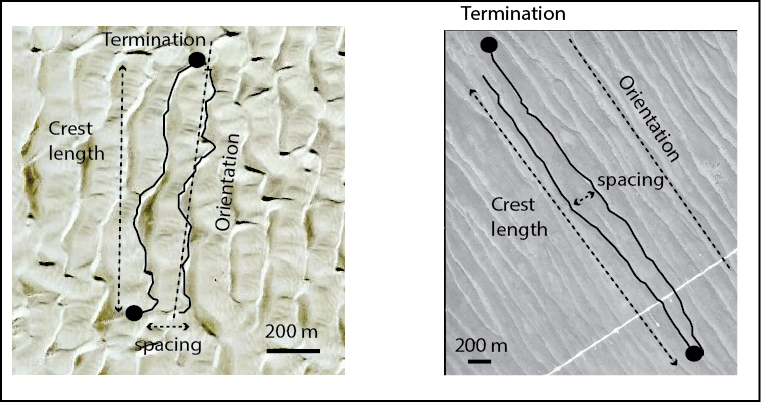
\includegraphics[width=\linewidth]{figures/dune_pattern_analysis}
	\caption{Examples of dune pattern analysis including metrics such as orientation, crest length, spacing, and termination points.}
	\label{fig:dune_pattern_metrics}
\end{figure}

\subsection{Challenges}

In order to automatically compute the metrics, the dune crest-lines must first be correctly detected and identified. Therefore, the bulk of the research presented will focus on crest-line detection, along with some general metrics calculations. Crest-lines can be defined as series of linear or curved segments, where all points along the segments represent the dune ridge line, and the ends of the segments represent the termination or defects in the pattern.

There are many ways to represent crest-lines. The most basic representation could be a vector which holds the trend or orientation (azimuth) and length. This representation is simplistic and can provide a general overview of the dune field. Sets of linear segments also facilitate the computation of some of the metrics desired. However, there are issues associated with the linear segments representation.

\begin{enumerate}
	\item Linear segments are only an approximate representation of the dune field and therefore there will be localization errors. In addition, dune crests are not always straight lines.
	\item The process of determining which linear segments are part of the actual crest-line can be difficult since there may be many false positives present in a given image.
	\item The data itself is quite noisy which will lead to many false positives in the detections.
	\item Computing accurate geomorphological metrics becomes challenging.
\end{enumerate}

A better representation would be a contiguous and smooth vector of two dimensional points which plot a curved segment, with the first and last points representing the location of the termination points. This is the representation which is favored and will be used as part of this research. The contiguous segment representation also provides a more accurate localization of dune crest-lines, and should produce more exact dune metric calculations.

Other challenges with automated crest-line detection are the algorithms and image processing tasks applied to the data sets. In satellite images of dune fields, the sun's orientation with respect to the image source greatly determines the appearance of the dunes. From an image representation perspective, a dune appears to have both a sunlit side, and a shaded side, as shown in Figure \ref{fig:intro_sample_images}. This translates to bright regions (large pixel values) for sunlit areas, and darker regions (low pixel values) for shaded areas. Crest-lines, or dune ridges, can the be defined to be the edge segments where the bright areas meet the darker areas in the image.

\begin{figure}
	\centering
	\begin{subfigure}{0.45\textwidth}
		\centering
		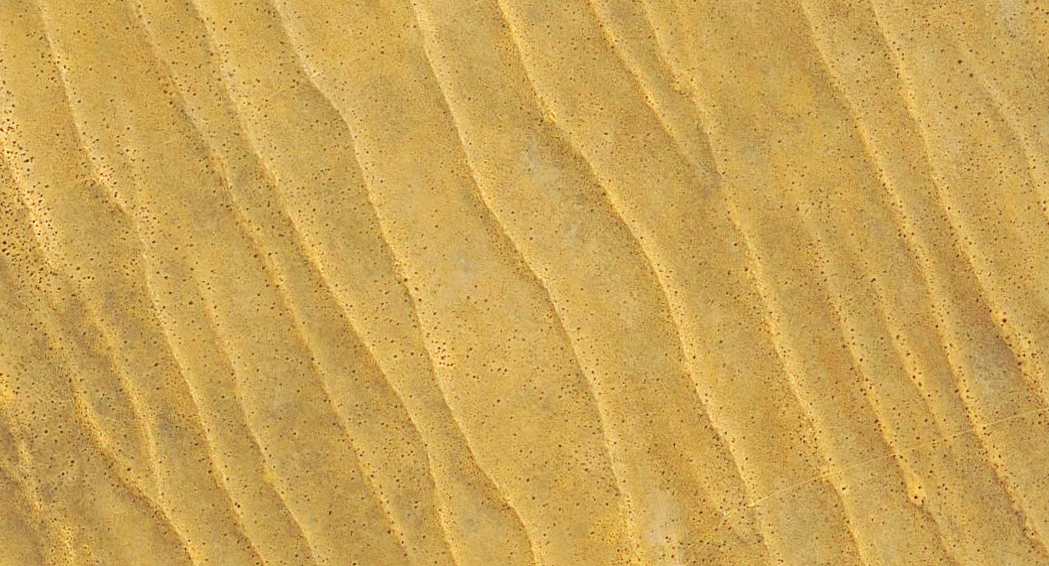
\includegraphics[width=\linewidth]{figures/kalahari}
		\caption{ Kalahari }
		\label{fig:intro_kalahari_image}
	\end{subfigure}
	\begin{subfigure}{0.45\textwidth}
		\centering
		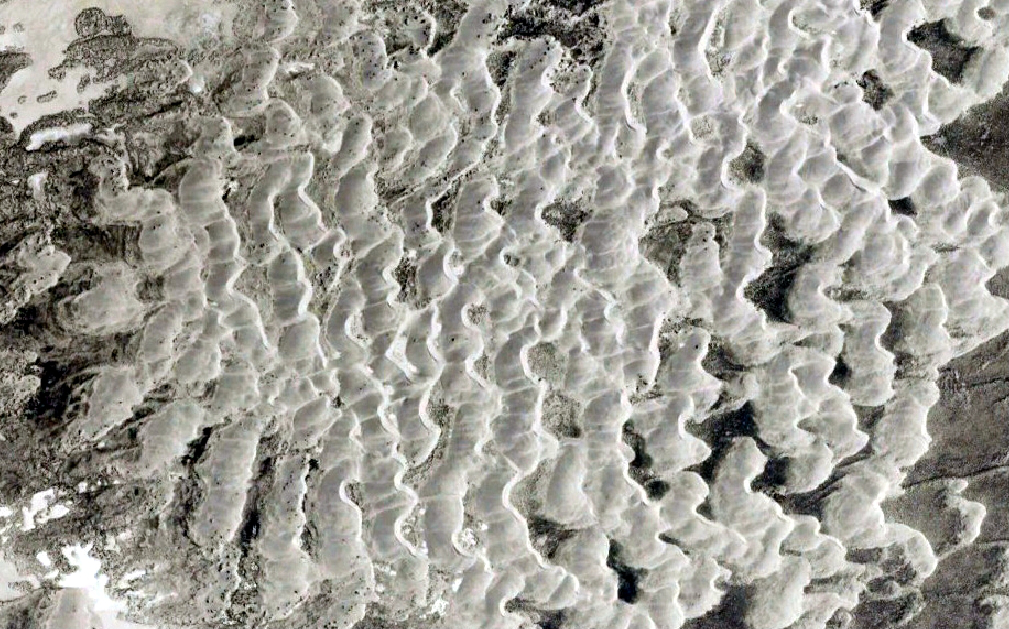
\includegraphics[width=\linewidth]{figures/wdc}
		\caption{ Winnemucca Dune Complex }
		\label{fig:intro_wdc_image}
	\end{subfigure}
	\caption{Sample satellite images of two distinct dune field regions: Kalahari and  Winnemucca Dune Complex }
	\label{fig:intro_sample_images}
\end{figure}

Issues arise when the sun's orientation is unknown, namely determining if an edge belongs to a crest-line ridge or is in fact a valley or the edge of a shadow. If the sun's orientation relative to the image is known, determining which edges are crest-lines or valleys becomes a much easier task. However, working under the assumption that the sun's relative orientation is unknown (which is the assumption made in this research), the ambiguity requires a resolution. In some cases, such as the Kalahari dune field shown in Figure \ref{fig:intro_kalahari_image}, determining the sun's orientation can be inferred from the image itself, since the dune ridges are relatively linear and well defined. On the other hand, in areas like the Winnemucca Dune Complex or WDC, shown in Figure \ref{fig:intro_wdc_image}, the sun's orientation cannot easily be determined. The factors which determine which edges are the crest-lines are not obvious, even for a human.

Another complexity which much be accounted for are the computer vision algorithms chosen to detect crest-lines. There are generally two approaches to solve these types of problems: appearance based and machine learning based approaches. Appearance-based approaches are typically fine tuned algorithms designed specifically to solve a problem set. The main drawback of these techniques are that they require significant manual tuning of parameters to achieve the desired accuracy to solve the problem. On the other hand, machine learning methods learn the problem set by example, and typically require many less parameters, which can be self optimized. Unfortunately, machine learning typically require a data set of training examples to construct the model to solve the problem. In this research, we explore both approaches using many different kinds of methods, specifically applied to the dune crest-line detection problem.

Once the crest-lines have been identified, the final challenge is computing the geomorphological properties of the dune fields. There are many levels of detail which can be computed for the metrics. At a coarse level, the global properties can be averaged for the entire dune field, while at a finer grain level, the metrics can be computed in local areas of the dune field around each crest-line. The latter is obviously more desirable, but requires more extensive and complex computations to accurately compute the desired metrics.

\subsection{Contributions}

The main contribution of this research is the development of a method to detect crest-lines from satellite images of planetary dune fields. The bulk of the research focuses on various regions on Earth, and the Ganges Chasma on Mars, also used in \cite{vaz_object_based_dune_analysis}. Each regions contains a data set of manually labeled satellite images, which includes all ground truth crest-lines.

A variety of methods were applied on each image set, and evaluated using the ground truth. Both appearance-based methods and machine learning are used to extract the crest-lines. The appearance-based method use a plethora of features such as intensity values, gradients, and frequency domain analysis, and other general image processing to attempt to find crest-lines. Machine learning methods are also used to construct models which can identify crest-line structures in the image. Each method is evaluated using the labeled ground truth, where the quality of each method is measured by precision and recall of the detected crest-lines, and the accuracy of the geomorphological metrics calculations. Each method has its own strengths and weaknesses, therefore the final proposed method combines both the edge-based and machine learning methods. 

The gradients in the image play an important role in discerning crest-lines. A critical piece of the algorithm is determining the dominant orientation of the dune field which is the overall trend of the dunes. It can be computed from the gradients of the crest-lines, which are affected by the sun's orientation relative to the dune field. 

Determining which gradients belong the the crest-lines and valleys is a challenging problem. A few solutions are proposed to solve this problem, including unsupervised methods such as K-Means, and normalized histograms of gradients. Once the dominant orientation gradients for crest-lines have been determined, the crest-lines can be more easily identified by keeping all gradients which \emph{agree} with the overall dominant orientation gradient.

Another important contribution is the \emph{gradient orientation map}. This maps the dot product of the gradients at each pixel with the computed dominant orientation gradient. In essence, pixels which \emph{agree} with the dominant orientation are emphasized separating shaded and bright sides of the dunes, which allows crest-lines to be easily traced.

The final proposed solution combines the dominant orientation, gradient orientation map, and a machine learning response map to find the crest-lines. The gradient based approach is used to extract initial candidate crest-lines. The response map is then used to both improve the localization of the crest-lines and to filter out false positive candidates.

A method for computing the dune field morphology metrics is also proposed. The main metrics computed are the overall orientation of the crest-lines, and the spacing between the crest-lines. The orientation is computed after crest-lines have been detected, which is done by quantizing the detected crest-lines into linear segments and computing the orientation of the lines. The dune spacing is computed by measuring the orthogonal distance between the lines.

The research is split into the following sections: the previous work and background is presented in section \ref{sec:background_perious_work}, which presents an overview of the study of dune fields, and work done in the field of image processing and computer vision, and previous dune detection implementations. In section \ref{sec:methodology}, the methodology is presented, included the various methods tried both for appearance-based, edge-based, and machine learning methods. It also presents the method for computing the geomorphological properties of a dune field. Section \ref{sec:experimental_evaluation} presents the  datasets used and the results of the detection and metrics for each approach. Finally, section \ref{sec:conclusion} discusses the methods and their results, along with proposing some future work on improving the approaches. 